%!TEX program = xelatex
%!BIB program = bibtex

\documentclass[en,black,12pt,normal]{elegantpaper}
\usepackage{float}
\usepackage{subfigure}
\usepackage{url}
\lstset{basicstyle=\footnotesize\ttfamily,frame=single}
\newcommand{\upcite}[1]{\textsuperscript{\textsuperscript{\cite{#1}}}}

\title{Final Report\\Revisit Metal-responsive transcription factor-1 (MTF-1)}
\author{WenYuan Jiang\\ID: 1951510\thanks{Undergraduate, F409, School of Life Science, Tongji University, Email: 1951510@tongji.edu.cn}}
\institute{School of Life Science, Tongji University}
%\version{1.00}
\date{May 7, 2021}
%\lstset{basicstyle=\footnotesize\ttfamily}
\AtBeginEnvironment{lstlisting}{\linespread{0.75}\selectfont}

\begin{document}

\maketitle
\begin{abstract}
\textbf{OBJECTIVE}: We want to demonstrate the skills learnt in this courses by performing a systematical bioinformatics analysis on teh gene MTF-1. We also aim to reproduce some of the analysis done by previous studies using the same data and similar techniques, and provide insight into this gene.\\
\textbf{RESULTS}: 1) equence of MTF-1 is conserved in different organisms. 2) MTF-1 may be an unstable hydrophilic protein. 3) MTF-1 has nuclear localization signal and zinc finger domains whichhelp it to bind metal response elements. 4) A consensus sequence named metal response elements can be foundin a certain set of genes. 5) Expression of a certain set of genes with metal response elements maybe regulated by MTF-1. \\
\textbf{CONCLUSION}: We successfully applied most of what we have learnt in this course to analyse the disease. The analysis indicates that platelet factor 4 in CD3+ cell is related to Aplastic Anemia, and the current immunosupressive treatment of this disease may not affect platelet factor 4 activity directly. 
\keywords{Metal-responsive transcription factor-1, \textit{in silico} analysis ,Coursework}
\end{abstract}
\section{Introduction}

In this paper, we will illustrate the skills we have learned from this course, by applying theories and analytical methods to study a gene named \textbf{MTF-1}.

The paper will first give an overview of MTF-1 and introduce the discovery of MTF-1 gene, which is mostly done in the 1990s by the people working in wet labs. Then, the methods used in this paper will be introduced. Next, results of some analysis using techniques taught in the course will be shown in detail, with steps given in the paper or in supplementary material. Finally, a discussion of the analysis and the results will be presented and we will be talking about issues like the merits and demerits of the methods, what the results indicates and how will these analysis inspire subsequent wet lab works.

Some of the contents of the paper will be based on previous studies, while others will be derived from the data and analysis, which could be inaccurate or misleading. We welcome any kind 
criticism of this paper.

\subsection{Overview of MTF-1}

MTF1 is the metal regulatory transcription factor 1.

In Homo sapiens (human), this gene encodes a transcription factor that induces expression of metallothioneins and other genes involved in metal homeostasis in response to heavy metals such as cadmium, zinc, copper, and silver. The protein is a nucleocytoplasmic shuttling protein that accumulates in the nucleus upon heavy metal exposure and binds to promoters containing a metal-responsive element (MRE).\upcite{ncbi:mtf1human}

\subsection{Discovery of the MTF-1}
In organisms, from the simple prokaryotic cells to complex vertebrate, metals plays an important role since many metal ions are involved in enzymatic reaction. 

The term heavy metal comprises a number of essential and nonessential metals. Among the latter cadmium, mercury and lead are toxic even in trace amounts. Although zinc and copper, which are essential heavy metals, are integral parts of proteins, notably enzymes and transcription factors, an excess of these metals is also toxic. Therefore, elaborate systems to import, sequester, store, transport and expel metals have evolved. Important players in metal homeostasis are the \textbf{metallothioneins}. These small proteins with a high content of cysteines can bind and thereby sequester heavy metals.\upcite{gunther2012taste}

\textbf{Metallothioneins} were discovered in 1957 by Margoshes and Vallee as cadmium-binding proteins in preparations of horse kidney.\upcite{margoshes1957cadmium} Transcription of metallothionein genes is upregulated in response to different stimuli, especially heavy metals. A hallmark of the promoters/enhancers of most metallothionein genes are short DNA sequence motifs termed metal response elements (MREs). The identification of these MREs, that share the core consensus sequence TGCRCNC (R=A or G, N= any nucleotide), suggested the existence of a specific transcription factor that regulates metallothionein expression in response to metals.\upcite{stuart1985identification} In 1988 a MRE-binding protein was identified by electrophoretic mobility shift and methylation interference studies.\upcite{westin1988zinc}\upcite{seguin1988detection} It is bound to its cognate DNA motif in a zinc dependent manner \upcite{westin1988zinc} and was termed MTF-1 (for MRE-binding transcription factor-1, more recently also metal-responsive transcription factor-1 or metal regulatory transcription factor-1). In 1993 the cDNA of mouse MTF-1 was cloned which revealed it as a zinc finger protein.\upcite{radtke1993cloned} Human MTF-1 with a length of 753 amino acids was cloned soon thereafter and found to be highly similar but slightly longer at the C-terminus than mouse MTF-1. \upcite{brugnera1994cloning}\upcite{gunther2012taste}
\section{Methods and data}

\subsection{Data source}
The sequence data is fetched from NCBI protein and nucleotide database, and the transcriptome dataset is fetched from NCBI GEO.

Detailed accession number are listed in Supplementary Material.

\subsection{Multiple sequence alignment}

Multiple sequence alignment is done using Clustal X version 2.1, with default parameters.
Visualization of multiple sequence alignment is done using R package ggmsa \url{https://github.com/YuLab-SMU/ggmsa}. The code is shown in the Supplementary Material.

\subsection{Phylogenetic tree building}
The phylogenetic tree is built using MegaX\upcite{kumar2018mega} Version 10.1.7. The algorithm of building the phylogenetic tree is the Maximum Likelihood algorithm, with parameters shown in the figure below.

\begin{figure}[H]
    \centering
    \includegraphics[width=0.5\textwidth]{image/MEGAX.png}
    \caption{Parameters of the phylogenetic tree building}
    \label{MEGAX}
\end{figure}

Then the phylogenetic tree is exported to a \texttt{.nwk} format and used in R for visualization.

\subsection{Protein physicochemical property prediction}
Protein physicochemical property prediction is done using Expasy ProtParam\upcite{gasteiger2005protein}. The complete sequence is analysed.
TMPred\upcite{hofmann1993tmbase} is also used to predict the hydrophobic region of proteins.
\subsection{Nuclear localization signal prediction}
Nuclear localization signal prediction is done using cNLS Mapper\upcite{kosugi2009systematic}, with a cut off set to 2.0.

\subsection{DNA binding site prediction for Cys2His2 zinc finger proteins}
DNA binding site prediction for Cys2His2 zinc finger proteins is done with the Interactive PWM predictor\upcite{persikov2014novo}, and the model used in this tool is expanded linear SVM\upcite{cortes1995support}.

\subsection{Transcriptome analysis}
Transcriptome analysis is done using the code derived from GEO2R. The grouping of the analysis is the same as the grouping in the GSE76510 data series.
\section{Results}

\subsection{Previous literature suggested a T cell-mediated autoimmune disorder of the hematopoietic system.}

Among all the 513 search results, there are 43 articles about aplastic anemia involves certain bioinformatics analysis, ranging from sequence comparison to transcriptomics analysis. 

All the 43 articles mentioned autoimmune disorder in most aplastic anemia cases, while 12 of them gives us an insight that T cell-mediated autoimmune disorder is closely related to aplastic anemia. Immune-mediated destruction of hematopoietic stem and progenitor cells is pathophysiologic in most cases of aplastic anemia (AA).\cite{zeng2004transcript}

The generated word cloud plot is shown below.

\begin{figure}[H]
    \centering
    \includegraphics[width=0.6\textwidth]{image/wordcloud.png}
    \caption{Selection standard}
    \label{WORD}
\end{figure}

We selected several articles involving the bioinfomatics skills we have learnt in this course as our data source to perform our analysis. The selected articles are listed in Supplementary Material section.


\subsection{Transcriptomics analysis of CD3+ T-cell reveals that platelet factor 4 is related to aplastic anemia pathophysiology.}

We fetched the data set GSE3807 from GEO. The data set is collected from 8 volunteers using Affymetrix Human Genome U133A Array (GPL96). Among the 8 samples, 6 are suffering from aplastic anemia, while the other 2 samples are from healthy control.\cite{franzke2006identification}

We identified the top 250 differently expressed genes from the data set, with the worst p value of 0.011. Using the differently expressed genes, we did a principal component analysis, and the result is shown below.

\begin{figure}[H]
    \centering
    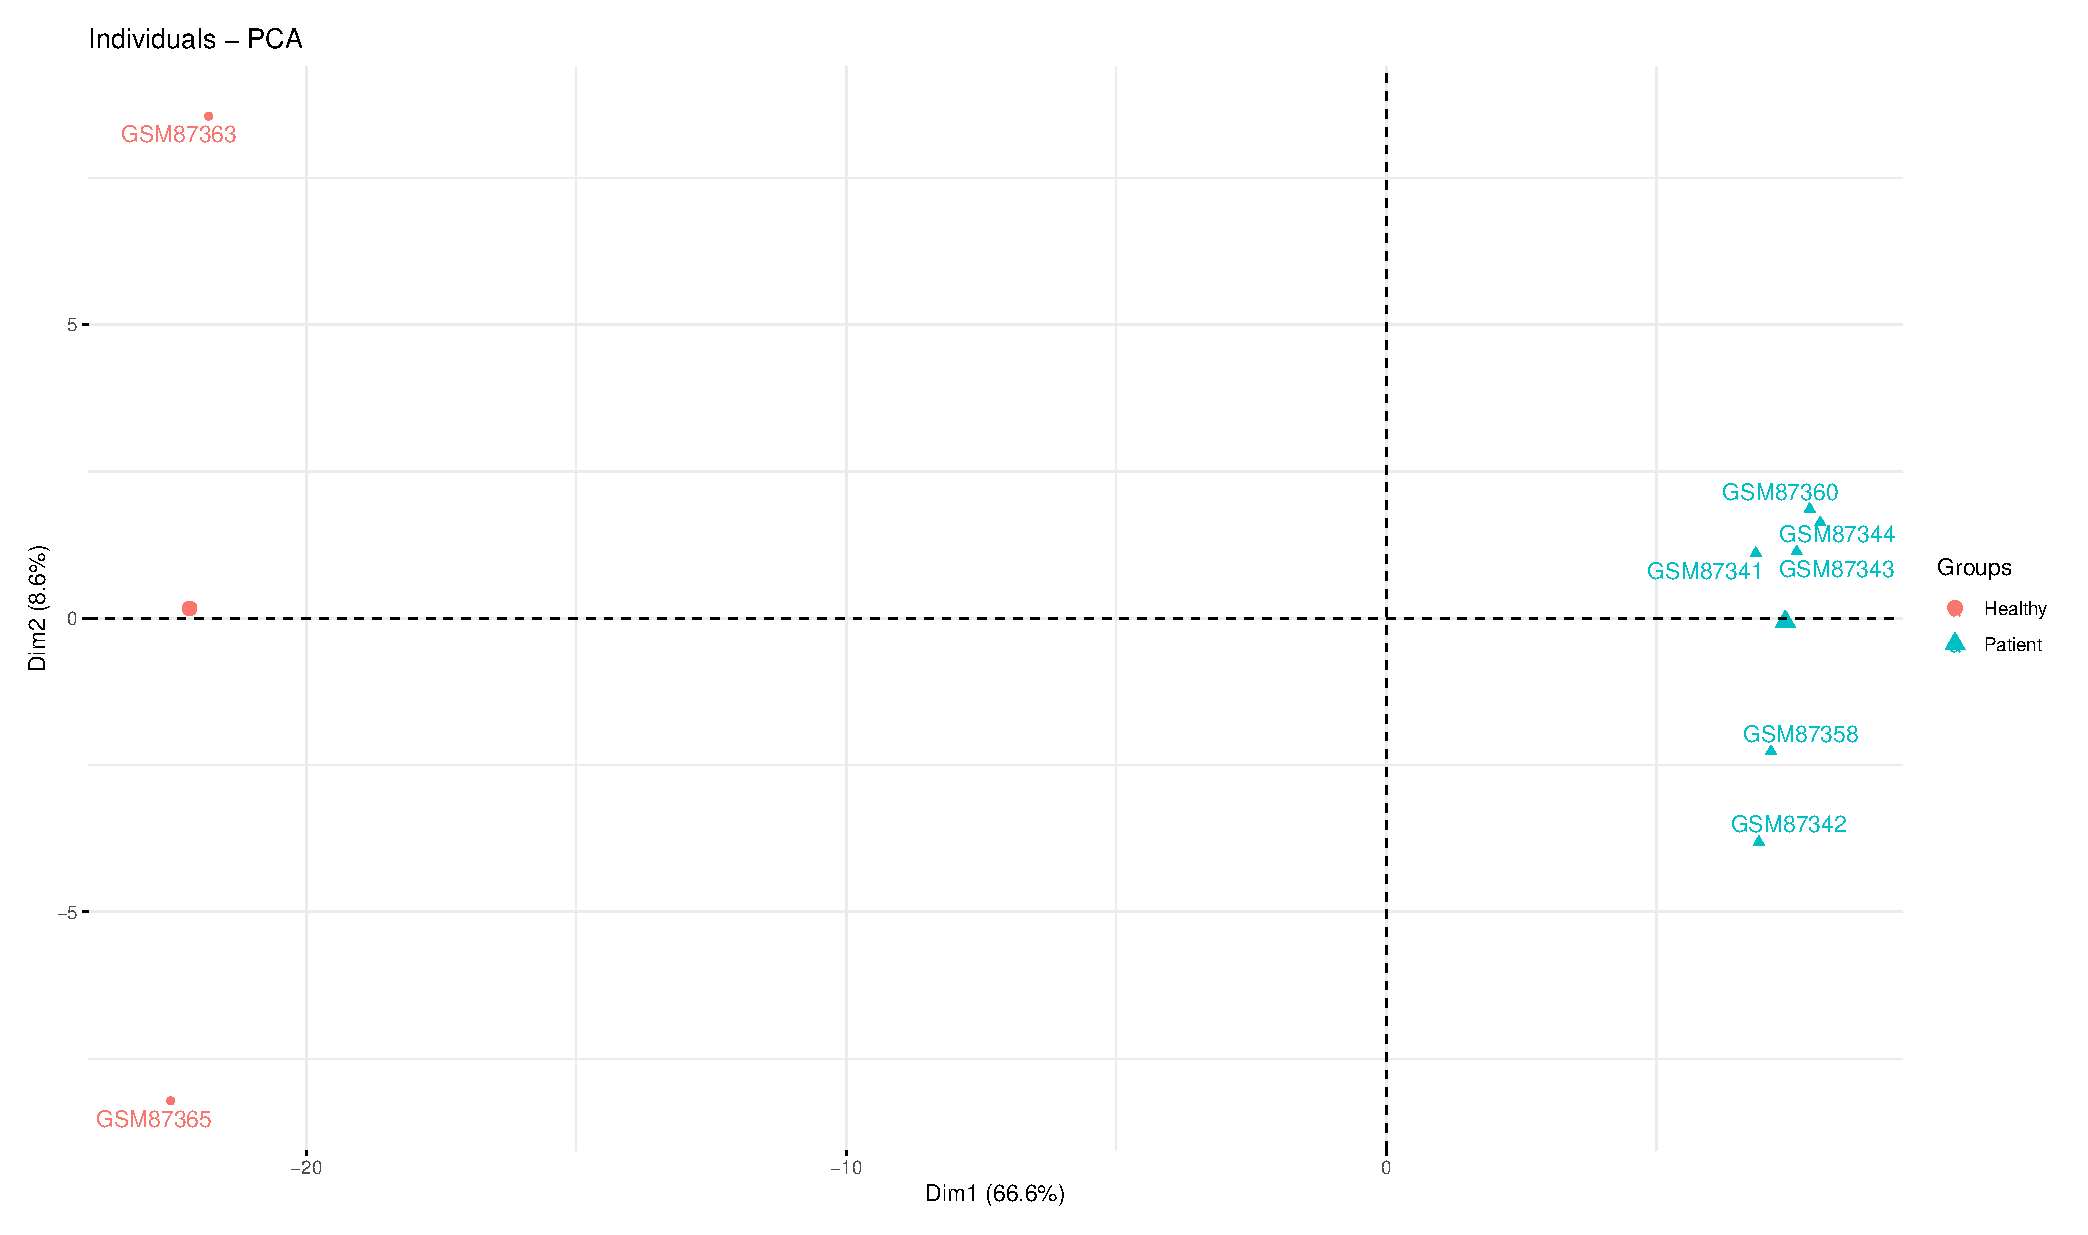
\includegraphics[width=0.9\textwidth]{image/PCACD31.eps}
    \caption{Result of principal component analysis}
    \label{PCACD3}
\end{figure}

PC1 and PC2 consist over 70\% of the principal components, which indicates that the analysis is desirable. According to the figure above, two groups of people are well separated by the PC1 and PC2 of the principal component analysis algorithm.

\begin{figure}[H]
    \centering
    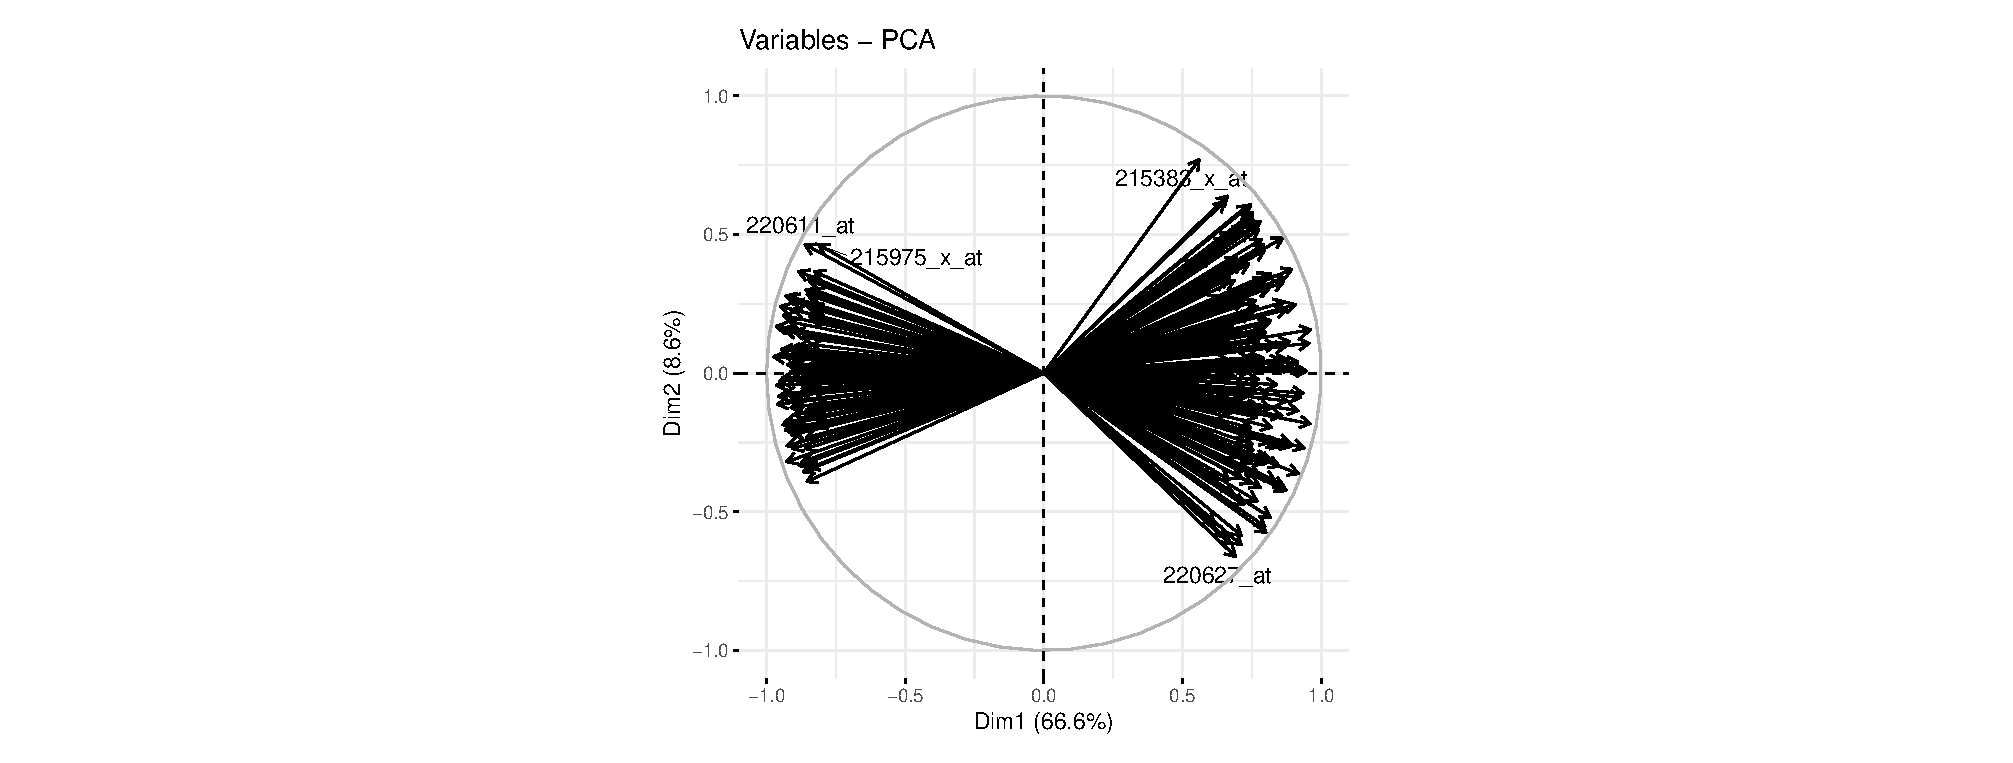
\includegraphics[width=0.5\textwidth]{image/PCAVCD3.eps}
    \caption{Variance of principal component analysis}
    \label{PCACD3}
\end{figure}


Heat map of the differently expressed genes is shown below.

\begin{figure}[H]
    \centering
    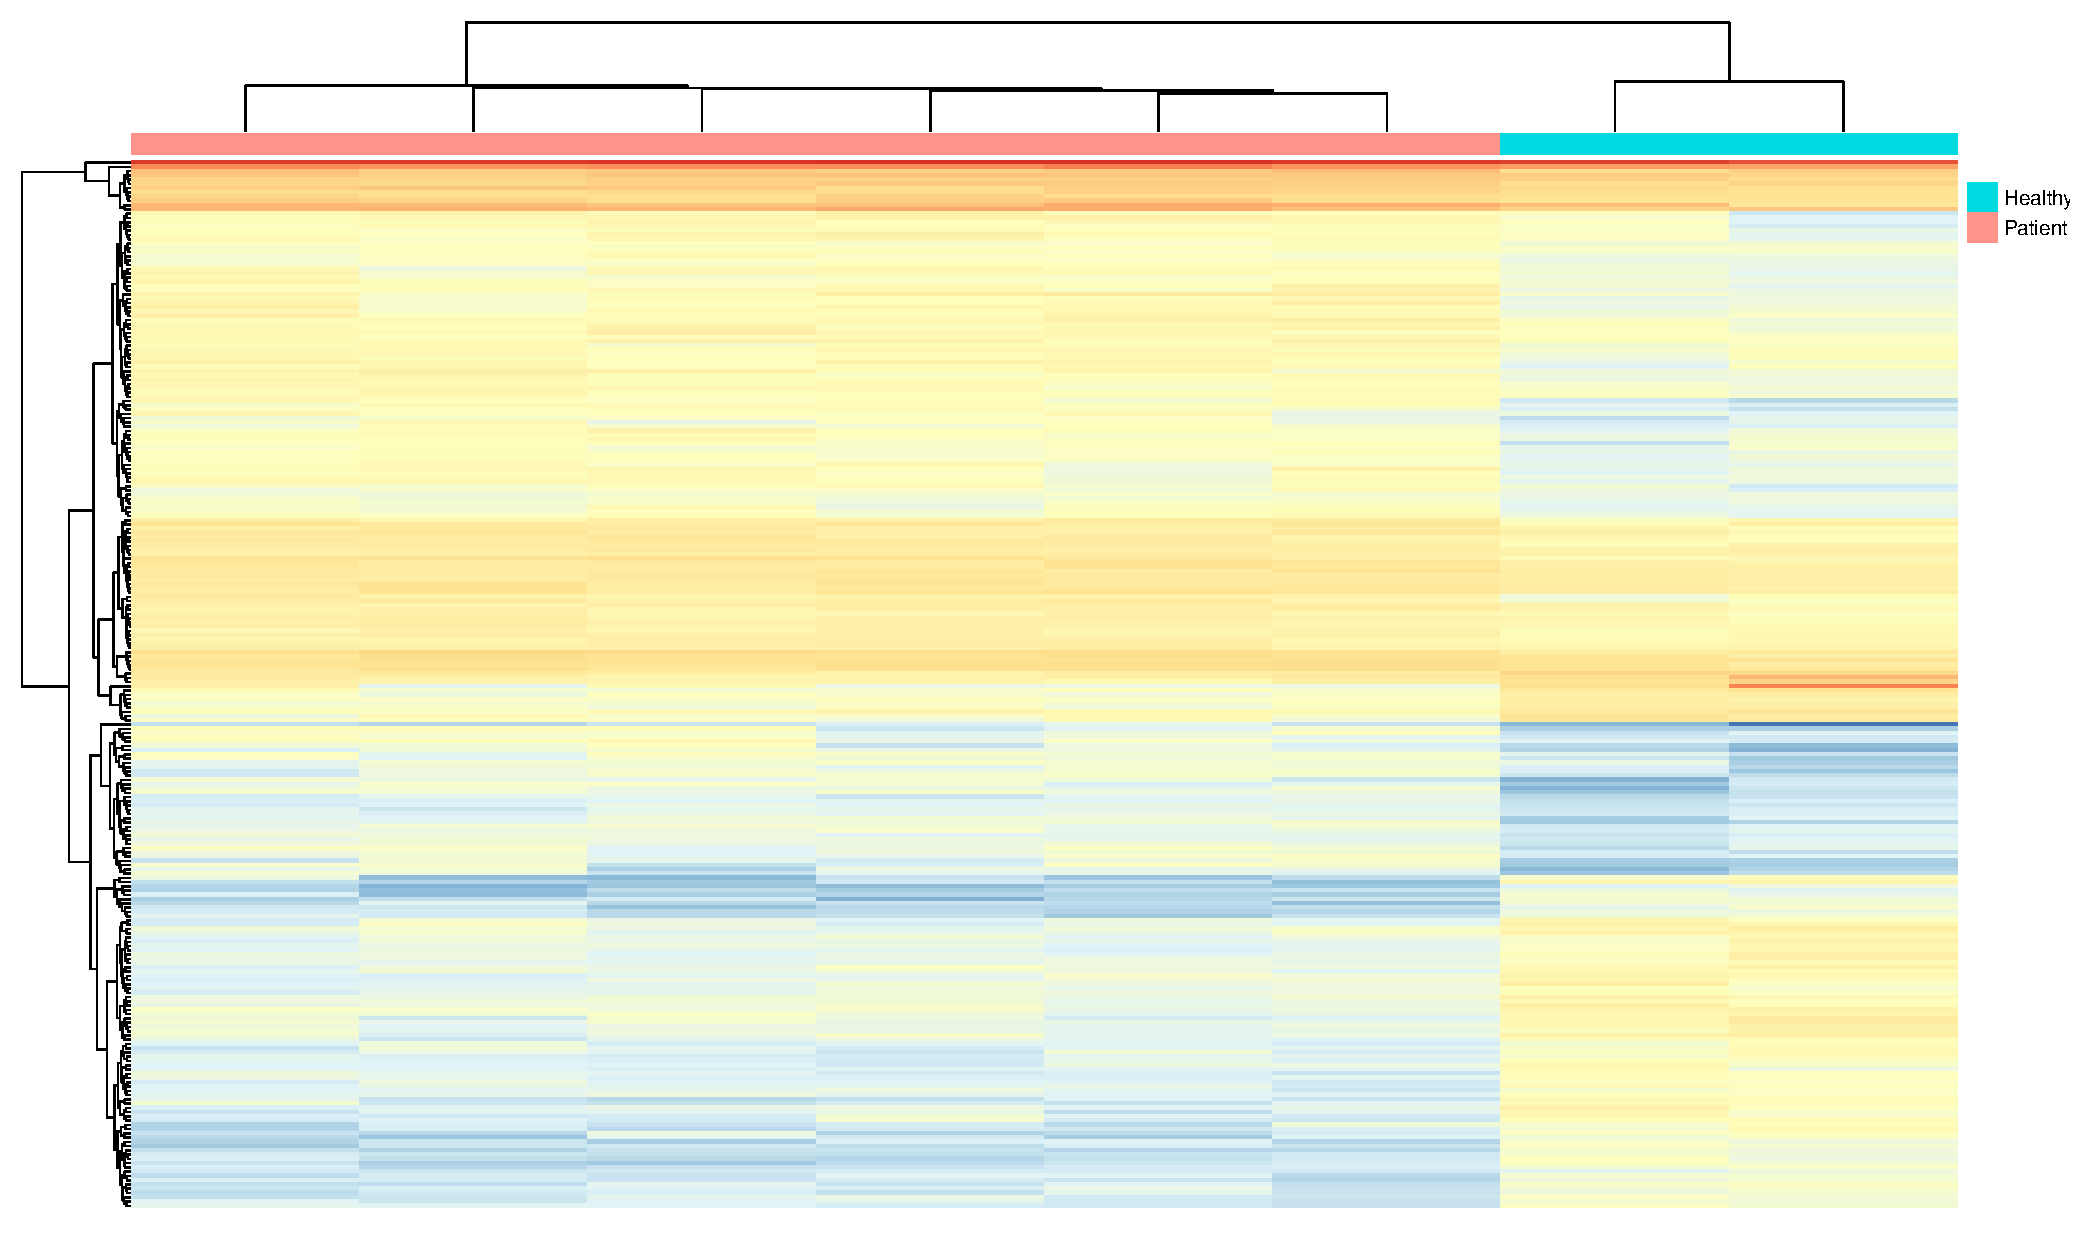
\includegraphics[width=0.9\textwidth]{image/HMCD3.eps}
    \caption{Heat map of the differently expressed genes}
    \label{HMCD3}
\end{figure}

From the heat map and the clustering results, clear divergence can be seen between the two groups. The main difference of the two groups are the genes that are down regulated in the Patients group, which is the lower-left part of the heat map.

To find out the functions of the down regulated genes, we did a GO enrichment on all down regulated genes, and the resulting dot plot is shown below.

\begin{figure}[H]
    \centering
    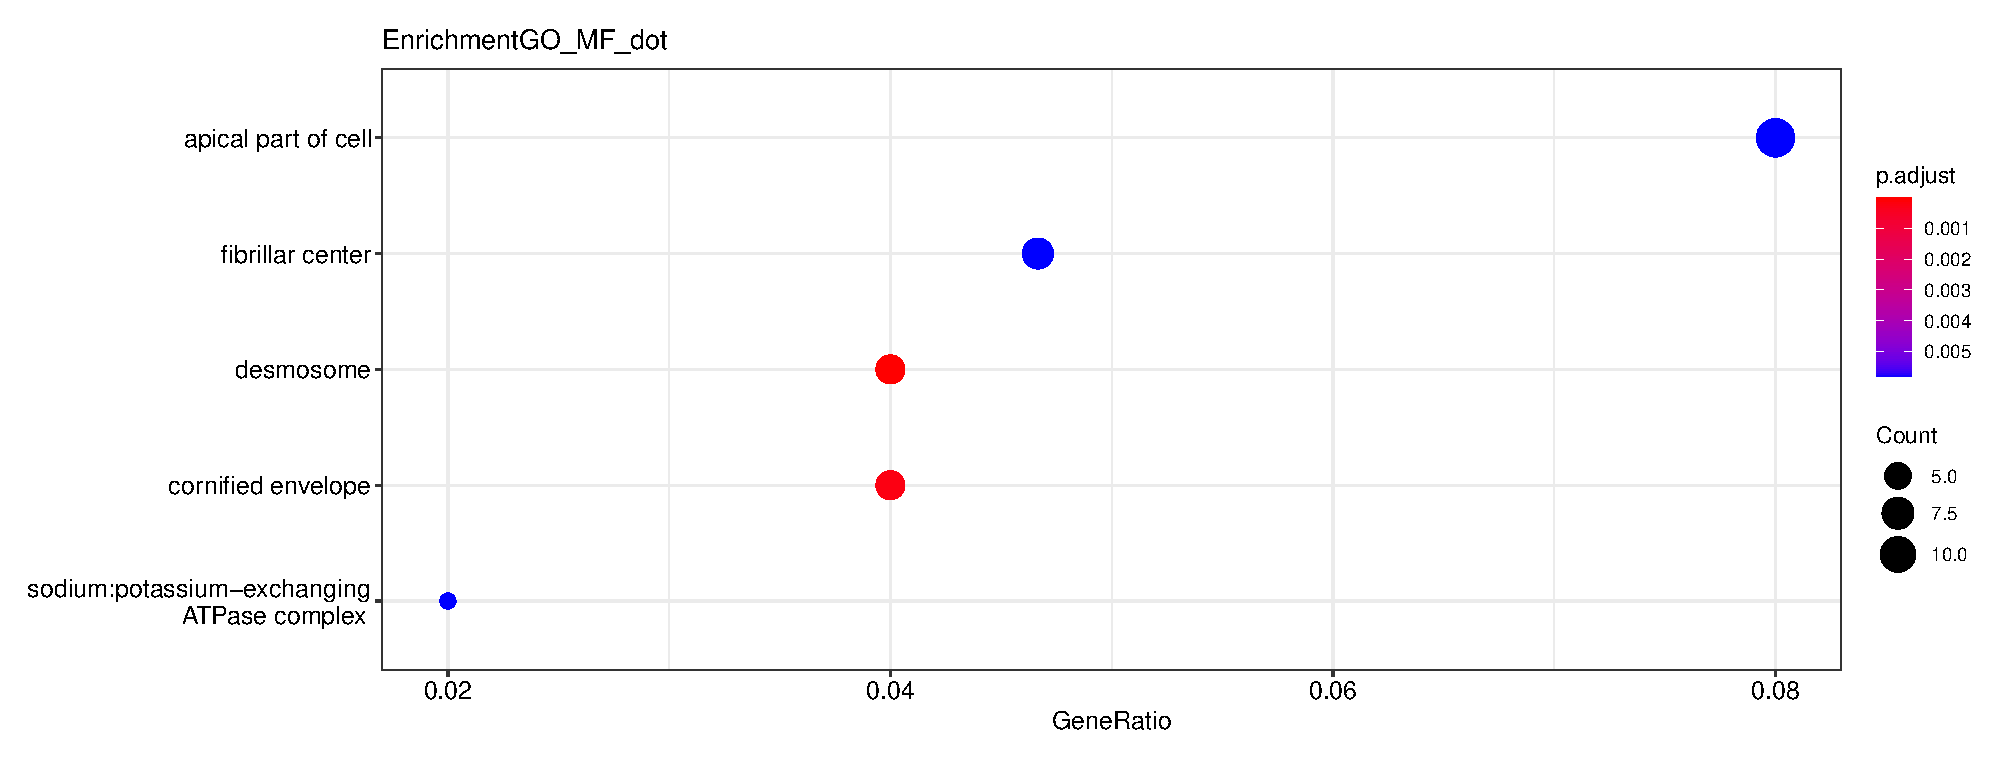
\includegraphics[width=1\textwidth]{image/EGOCD3.eps}
    \caption{GO enrichment of down regulated genes}
    \label{HMCD3}
\end{figure}

Among the down regulated genes, one gene named platelet factor 4 (PF4) caught our attention. PF4 is 27 folds lower in the patients group than in healthy control, and the p value of the gene is 0.005. Considering that PF4 is closely related to platelet formation and functions, we can say that platelet factor 4 is related to aplastic anemia pathophysiology.

\subsection{Platelet factor 4 has sequence homology with some chemokine family members.}

We fetched the sequence of Platelet factor 4, and run a psi-blast against the NCBI protein database, and the organism is limited to human. The results are then analysed using ClustalX 2.1 to perform an MSA.

\begin{figure}[H]
    \centering
    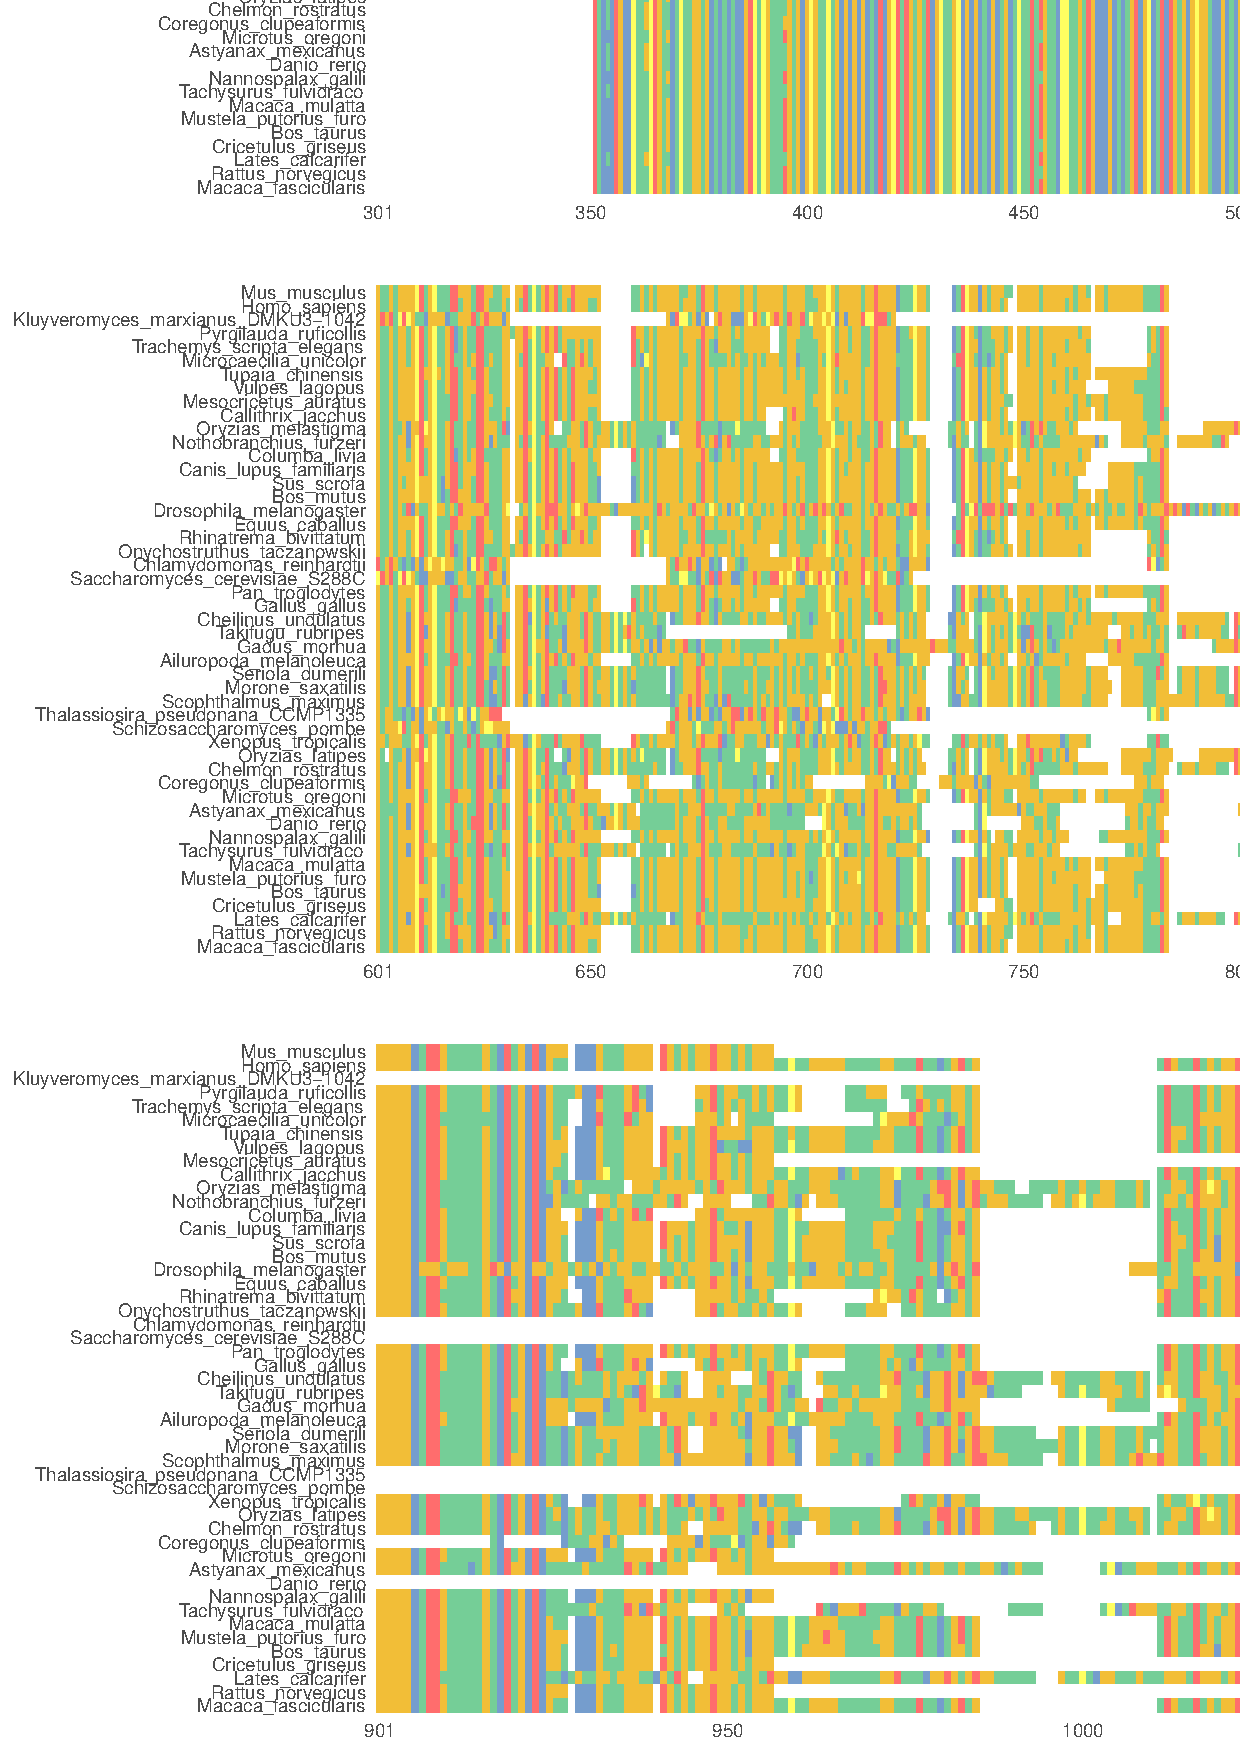
\includegraphics[width=1\textwidth]{image/MSA.png}
    \caption{MSA results}
    \label{HMCD3}
\end{figure}

According to the MSA results, A consensus pattern named C-X-C motif can be found in PF4 (NP\_002611.1). The hits indicated a conserved domain that classifies the PF4 into CXC family chemokine, which is a chemotactic factor that attracts neutrophils, basophils, and T-cells, but not monocytes, and is involved in neutrophil activation.

\begin{figure}[H]
    \centering
    \includegraphics[width=1\textwidth]{image/PF4D.png}
    \caption{Conserved domain of Platelet factor 4}
    \label{HMCD3}
\end{figure}

Visualization of the PF4 is shown in the figure below. The purple colored part is the C-X-C motif.

\begin{figure}[H]
    \centering
    \includegraphics[width=1\textwidth]{image/PF43D2.png}
    \caption{Structure and Conserved domain of Platelet factor 4}
    \label{HMCD3}
\end{figure}

According to previous literature, platelet factor 4 (PF4) is a small cytokine belonging to the CXC chemokine family that is also known as chemokine (C-X-C motif) ligand 4 (CXCL4). This chemokine is released from alpha-granules of activated platelets during platelet aggregation, and promotes blood coagulation by moderating the effects of heparin-like molecules. Due to these roles, it is predicted to play a role in wound repair and inflammation. It is usually found in a complex with proteoglycan.\cite{fernandez2002structure}

\subsection{Platelet factor 4 and other CXC chemokine related genes are differently expressed in CD3+ T-cell of aplastic anemia patients.}

Among all the genes that are related to CXC chemokine family, 34 of them are measured on the micro array. There are 24 of the 34 relevant genes are down regulated in the patient group compared with the healthy control, while others are slightly up regulated. The differently expressed CXC chemokine related genes and their logFC values are demonstrated in the heat map below.

\begin{figure}[H]
    \centering
    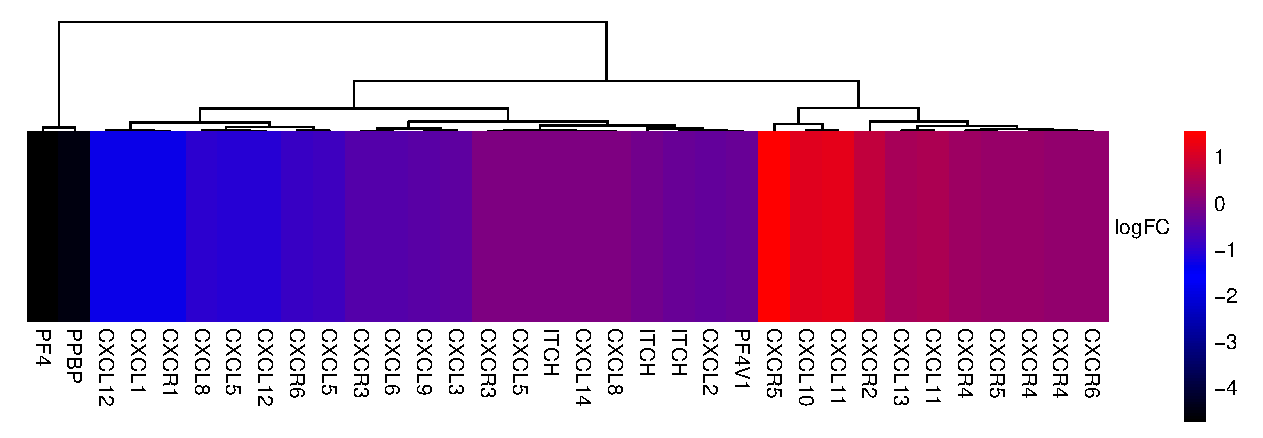
\includegraphics[width=1\textwidth]{image/CXCHM.eps}
    \caption{Structure and Conserved domain of Platelet factor 4}
    \label{HMCD3}
\end{figure}

\subsection{Platelet factor 4 is cleaved into a short form and binds heparin with high affinity.}

We queried the Nextprot database for more detailed information about Platelet factor 4. The platelet factor 4 has its signal peptide cut to form the mature protein, and the mature protein is cleaved into a short form, which can bind strongly to heparin. The figure below shows the sequence features of Platelet factor 4.

\begin{figure}[H]
    \centering
    \includegraphics[width=1\textwidth]{image/PF4ISO.png}
    \caption{Sequence features of Platelet factor 4}
    \label{HMCD3}
\end{figure}

According to the GO annotation of platelet factor 4 in the database, it has high affinity to bind heparin, and we did a molecular docking to confirm this claim \textit{in silico}. 

The lowest energy conformation is shown in the figure below.

\begin{figure}[H]
    \centering
    \includegraphics[width=0.7\textwidth]{image/DOCK.png}
    \caption{Lowest energy docking conformation}
    \label{HMCD3}
\end{figure}

\begin{lstlisting}
REMARK  Energy: -17.5306
REMARK  SimpleFitness: -17.5306
REMARK  FullFitness: -2058.942
REMARK  InterFull: -308.048
REMARK  IntraFull: 42.5802
REMARK  solvFull: -1990.93
REMARK  surfFull: 197.456
REMARK  extraFull: 0.0
REMARK  deltaGcompsolvpol: -1990.93
REMARK  deltaGcompsolvnonpol: 197.456
REMARK  deltaGprotsolvpol: -2104.32
REMARK  deltaGprotsolvnonpol: 195.666
REMARK  deltaGligsolvpol: -171.412
REMARK  deltaGligsolvnonpol: 12.8132
REMARK  deltaGvdw: -308.048
REMARK  deltaGelec: 0.0
REMARK  deltaG: -16.744253
REMARK  Cluster: 0
REMARK  ClusterRank: 0
\end{lstlisting}





\subsection{Immunosupressive agent Prednisone has less affinity to PF4, compared with heparin.}

We also docked commonly used immunosupressive agents like Prednisone, Cyclosporin and Tacrolimus, which are used in immunosupressive therapies, but they showed little affinity to PF4, compared with heparin.

The docking result of Prednisone is shown below.

\begin{figure}[H]
    \centering
    \includegraphics[width=0.7\textwidth]{image/DOCK2.png}
    \caption{Lowest energy docking conformation}
    \label{HMCD3}
\end{figure}

\begin{lstlisting}
REMARK  Energy: 26.0314
REMARK  SimpleFitness: 26.0314
REMARK  FullFitness: -1853.696
REMARK  InterFull: -36.5928
REMARK  IntraFull: 81.3677
REMARK  solvFull: -2095.95
REMARK  surfFull: 197.479
REMARK  extraFull: 0.0
REMARK  deltaGcompsolvpol: -2095.95
REMARK  deltaGcompsolvnonpol: 197.479
REMARK  deltaGprotsolvpol: -2104.32
REMARK  deltaGprotsolvnonpol: 195.666
REMARK  deltaGligsolvpol: -17.0954
REMARK  deltaGligsolvnonpol: 11.6588
REMARK  deltaGvdw: -36.5928
REMARK  deltaGelec: 0.0
REMARK  deltaG: -6.8246017
REMARK  Cluster: 0
REMARK  ClusterRank: 0

\end{lstlisting}

The optimal conformation in the figure above has -6.82 Estimated $\delta$G (kcal/mol) which is relatively weak. This indicates that Prednisone as an immunosupressive agent, may not be directly affecting the function of PF4.

\section{Discussion \& Conclusions}

We started our analysis from the multiple sequence alignment of MTF-1 protein sequence in different organisms and find out that protein sequence of MTF-1 is conserved in different organisms. We then analysed the nucleotide sequence of MTF-1, and found that the exon and intron patterns share a high similarity among these organisms.

Similar sequence indicates that similar feathers and functions exist. Therefore we did analysis on the physicochemical properties of MTF-1 in in different organisms, and the results are consistent with our initial guess.

To study the function of MTF-1, we first checked the sequence for special domains. Nuclear localization signal and Zinc finger domain are found, which suggests that MTF-1 works like a transcription factor. Since the zinc finger domains can recognize and bind to specific DNA sequences, we would like to know what the target sequences are. Fortunately, suitable tools are published and we are able to get the consensus sequence of MTF-1 target/binding sequences.

With the MTF-1 target/binding sequences, the question about what genes are regulated via the MTF-1 target/binding sequences (that is, metal response elements MREs) formed. Through sequence screening and transcriptome analysis, several genes that are likely to be regulated by MTF-1 is found.

Still, we do not know the exact structure of the MTF-1, since homologous modeling of MTF-1 fails to give out reasonable structures. \textit{Ab initio} methods, however, cost too much time and computation resources for facilities to afford. Considering that MTF-1 is an unstable protein, elucidation opf its structure by X-ray crystallography may face difficulties, and other methods, like NMR, is not suitable for such a large protein. Cryoelectron Microscopy might be a choice for this task, butin our literature review, no relevant work was found.

If we have the exact structure of the MTF-1, many processes involving MTF-1 will be studied more deeply, and we can gain more insight into the mechanisms of metal regulatory transcription factor, including but not limited to MTF-1.
\section{Acknowledgment}

Throughout the writing of this report I have received a great deal of support and assistance.

I would like to thank the teachers of the course, whose expertise was invaluable in formulating the research questions and methodology. 

I would also like to acknowledge my classmates in this course for their wonderful collaboration. I would particularly like to single out Zhifan Lin, I want to thank you for your patient support and insightful suggestions.

\section*{Supplementary Material}

\subsection*{Accession number of sequences and GEO data set}
The accession number of sequences are listed below.
\begin{lstlisting}[basicstyle=\tiny\ttfamily]
>NP_032662.3 Mtf1 [organism=Mus musculus] [GeneID=17764]
>NP_001097560.1 MTF-1 [organism=Drosophila melanogaster] [GeneID=39089] [isoform=C ]
>NP_001097561.1 MTF-1 [organism=Drosophila melanogaster] [GeneID=39089] [isoform=D ]
>NP_001097562.1 MTF-1 [organism=Drosophila melanogaster] [GeneID=39089] [isoform=E ]
>NP_001287002.1 MTF-1 [organism=Drosophila melanogaster] [GeneID=39089] [isoform=F ]
>NP_001287003.1 MTF-1 [organism=Drosophila melanogaster] [GeneID=39089] [isoform=G ]
>NP_648311.2 MTF-1 [organism=Drosophila melanogaster] [GeneID=39089] [isoform=A ]
>NP_729491.1 MTF-1 [organism=Drosophila melanogaster] [GeneID=39089] [isoform=B ]
>NP_001027866.1 mtf1 [organism=Takifugu rubripes] [GeneID=446075]
>XP_029694032.1 mtf1 [organism=Takifugu rubripes] [GeneID=446075] [isoform=X1]
>XP_029694033.1 mtf1 [organism=Takifugu rubripes] [GeneID=446075] [isoform=X1]
>XP_029694034.1 mtf1 [organism=Takifugu rubripes] [GeneID=446075] [isoform=X2]
>XP_029694035.1 mtf1 [organism=Takifugu rubripes] [GeneID=446075] [isoform=X3]
>XP_029694036.1 mtf1 [organism=Takifugu rubripes] [GeneID=446075] [isoform=X4]
>XP_029694037.1 mtf1 [organism=Takifugu rubripes] [GeneID=446075] [isoform=X5]
>XP_029694038.1 mtf1 [organism=Takifugu rubripes] [GeneID=446075] [isoform=X6]
>XP_029694039.1 mtf1 [organism=Takifugu rubripes] [GeneID=446075] [isoform=X7]
>NP_005946.2 MTF1 [organism=Homo sapiens] [GeneID=4520]
>XP_011539793.1 MTF1 [organism=Homo sapiens] [GeneID=4520] [isoform=X1]
>XP_011539795.1 MTF1 [organism=Homo sapiens] [GeneID=4520] [isoform=X2]
>XP_011539796.1 MTF1 [organism=Homo sapiens] [GeneID=4520] [isoform=X3]
>NP_013955.1 MTF1 [organism=Saccharomyces cerevisiae S288C] [GeneID=855268]
>XP_027004713.1 mtf1 [organism=Tachysurus fulvidraco] [GeneID=113644242] [isoform=X1]
>XP_027004715.1 mtf1 [organism=Tachysurus fulvidraco] [GeneID=113644242] [isoform=X2]
>XP_027004716.1 mtf1 [organism=Tachysurus fulvidraco] [GeneID=113644242] [isoform=X3]
>XP_027004717.1 mtf1 [organism=Tachysurus fulvidraco] [GeneID=113644242] [isoform=X3]
>XP_027004718.1 mtf1 [organism=Tachysurus fulvidraco] [GeneID=113644242] [isoform=X3]
>NP_694513.1 mtf1 [organism=Danio rerio] [GeneID=195821]
>XP_021322285.1 mtf1 [organism=Danio rerio] [GeneID=195821] [isoform=X1]
>XP_021322286.1 mtf1 [organism=Danio rerio] [GeneID=195821] [isoform=X2]
>NP_593495.1 mtf1 [organism=Schizosaccharomyces pombe] [GeneID=2543271]
>NP_001102147.1 Mtf1 [organism=Rattus norvegicus] [GeneID=362591]
>XP_006238946.1 Mtf1 [organism=Rattus norvegicus] [GeneID=362591] [isoform=X1]
>XP_038966270.1 Mtf1 [organism=Rattus norvegicus] [GeneID=362591] [isoform=X2]
>XP_038966271.1 Mtf1 [organism=Rattus norvegicus] [GeneID=362591] [isoform=X3]
>XP_038966272.1 Mtf1 [organism=Rattus norvegicus] [GeneID=362591] [isoform=X4]
>NP_001026666.1 MTF1 [organism=Gallus gallus] [GeneID=428218]
>XP_015153181.1 MTF1 [organism=Gallus gallus] [GeneID=428218] [isoform=X2]
>XP_040507666.1 MTF1 [organism=Gallus gallus] [GeneID=428218] [isoform=X1]
>XP_040507667.1 MTF1 [organism=Gallus gallus] [GeneID=428218] [isoform=X1]
>NP_001267060.1 MTF1 [organism=Pan troglodytes] [GeneID=456766]
>XP_009451322.1 MTF1 [organism=Pan troglodytes] [GeneID=456766] [isoform=X1]
>XP_016806813.1 MTF1 [organism=Pan troglodytes] [GeneID=456766] [isoform=X1]
>XP_016806894.1 MTF1 [organism=Pan troglodytes] [GeneID=456766] [isoform=X3]
>XP_024202793.1 MTF1 [organism=Pan troglodytes] [GeneID=456766] [isoform=X2]
>NP_001030252.2 MTF1 [organism=Bos taurus] [GeneID=509960]
>XP_005204750.1 MTF1 [organism=Bos taurus] [GeneID=509960] [isoform=X1]
>NP_001244724.1 MTF1 [organism=Macaca mulatta] [GeneID=714795]
>XP_014991031.1 MTF1 [organism=Macaca mulatta] [GeneID=714795] [isoform=X1]
>XP_014991038.1 MTF1 [organism=Macaca mulatta] [GeneID=714795] [isoform=X1]
>XP_028701043.1 MTF1 [organism=Macaca mulatta] [GeneID=714795] [isoform=X2]
>XP_002291569.1 MTF1 [organism=Thalassiosira pseudonana CCMP1335] [GeneID=7442748]
>XP_002939525.1 mtf1 [organism=Xenopus tropicalis] [GeneID=100495484]
>XP_012812846.1 mtf1 [organism=Xenopus tropicalis] [GeneID=100495484]
>XP_031752770.1 mtf1 [organism=Xenopus tropicalis] [GeneID=100495484]
>XP_004740804.1 MTF1 [organism=Mustela putorius furo] [GeneID=101690205] [isoform=X1]
>XP_004740805.1 MTF1 [organism=Mustela putorius furo] [GeneID=101690205] [isoform=X2]
>XP_005543973.1 MTF1 [organism=Macaca fascicularis] [GeneID=101926816]
>XP_005543974.1 MTF1 [organism=Macaca fascicularis] [GeneID=101926816]
>XP_005543975.1 MTF1 [organism=Macaca fascicularis] [GeneID=101926816]
>XP_001703129.1 MTF1 [organism=Chlamydomonas reinhardtii] [GeneID=5728690]
>XP_005628986.1 MTF1 [organism=Canis lupus familiaris] [GeneID=608127] [isoform=X3]
>XP_005628987.1 MTF1 [organism=Canis lupus familiaris] [GeneID=608127] [isoform=X3]
>XP_013975033.1 MTF1 [organism=Canis lupus familiaris] [GeneID=608127] [isoform=X2]
>XP_022283522.1 MTF1 [organism=Canis lupus familiaris] [GeneID=608127] [isoform=X1]
>XP_038351419.1 MTF1 [organism=Canis lupus familiaris] [GeneID=608127] [isoform=X1]
>XP_038351420.1 MTF1 [organism=Canis lupus familiaris] [GeneID=608127] [isoform=X2]
>XP_038351421.1 MTF1 [organism=Canis lupus familiaris] [GeneID=608127] [isoform=X3]
>XP_038351422.1 MTF1 [organism=Canis lupus familiaris] [GeneID=608127] [isoform=X3]
>XP_038413769.1 MTF1 [organism=Canis lupus familiaris] [GeneID=608127] [isoform=X1]
>XP_038413770.1 MTF1 [organism=Canis lupus familiaris] [GeneID=608127] [isoform=X2]
>XP_038413771.1 MTF1 [organism=Canis lupus familiaris] [GeneID=608127] [isoform=X3]
>XP_038413772.1 MTF1 [organism=Canis lupus familiaris] [GeneID=608127] [isoform=X3]
>XP_038477644.1 MTF1 [organism=Canis lupus familiaris] [GeneID=608127] [isoform=X1]
>XP_038477645.1 MTF1 [organism=Canis lupus familiaris] [GeneID=608127] [isoform=X2]
>XP_038477646.1 MTF1 [organism=Canis lupus familiaris] [GeneID=608127] [isoform=X3]
>XP_038477647.1 MTF1 [organism=Canis lupus familiaris] [GeneID=608127] [isoform=X3]
>XP_038543415.1 MTF1 [organism=Canis lupus familiaris] [GeneID=608127] [isoform=X1]
>XP_038543416.1 MTF1 [organism=Canis lupus familiaris] [GeneID=608127] [isoform=X2]
>XP_038543417.1 MTF1 [organism=Canis lupus familiaris] [GeneID=608127] [isoform=X3]
>XP_038543418.1 MTF1 [organism=Canis lupus familiaris] [GeneID=608127] [isoform=X3]
>XP_011228926.1 MTF1 [organism=Ailuropoda melanoleuca] [GeneID=100480003] [isoform=X2]
>XP_034505425.1 MTF1 [organism=Ailuropoda melanoleuca] [GeneID=100480003] [isoform=X1]
>XP_034505435.1 MTF1 [organism=Ailuropoda melanoleuca] [GeneID=100480003] [isoform=X3]
>XP_034505440.1 MTF1 [organism=Ailuropoda melanoleuca] [GeneID=100480003] [isoform=X4]
>NP_001230473.1 MTF1 [organism=Sus scrofa] [GeneID=100511998]
>XP_020948959.1 MTF1 [organism=Sus scrofa] [GeneID=100511998] [isoform=X1]
>XP_020948960.1 MTF1 [organism=Sus scrofa] [GeneID=100511998] [isoform=X2]
>XP_005084415.1 Mtf1 [organism=Mesocricetus auratus] [GeneID=101832232] [isoform=X1]
>XP_012979330.1 Mtf1 [organism=Mesocricetus auratus] [GeneID=101832232] [isoform=X2]
>XP_005509709.1 MTF1 [organism=Columba livia] [GeneID=102092487]
>XP_006158647.1 MTF1 [organism=Tupaia chinensis] [GeneID=102475717] [isoform=X1]
>XP_006158648.1 MTF1 [organism=Tupaia chinensis] [GeneID=102475717] [isoform=X2]
>XP_014447108.1 MTF1 [organism=Tupaia chinensis] [GeneID=102475717] [isoform=X3]
>XP_027255030.1 Mtf1 [organism=Cricetulus griseus] [GeneID=100752132] [isoform=X3]
>XP_035295521.1 Mtf1 [organism=Cricetulus griseus] [GeneID=100752132]
>XP_035295522.1 Mtf1 [organism=Cricetulus griseus] [GeneID=100752132]
>XP_035311622.1 Mtf1 [organism=Cricetulus griseus] [GeneID=100752132] [isoform=X1]
>XP_005893304.1 MTF1 [organism=Bos mutus] [GeneID=102267771]
>XP_008848440.2 Mtf1 [organism=Nannospalax galili] [GeneID=103747698]
>XP_035479853.1 mtf1 [organism=Scophthalmus maximus] [GeneID=118299875] [isoform=X1]
>XP_035479862.1 mtf1 [organism=Scophthalmus maximus] [GeneID=118299875] [isoform=X1]
>XP_035479869.1 mtf1 [organism=Scophthalmus maximus] [GeneID=118299875] [isoform=X2]
>XP_022676757.1 MTF1 [organism=Kluyveromyces marxianus DMKU3-1042] [GeneID=34716899]
>XP_018554070.1 mtf1 [organism=Lates calcarifer] [GeneID=108898617] [isoform=X1]
>XP_018554076.1 mtf1 [organism=Lates calcarifer] [GeneID=108898617] [isoform=X2]
>XP_022619994.1 mtf1 [organism=Seriola dumerili] [GeneID=111235748]
>XP_024122982.1 mtf1 [organism=Oryzias melastigma] [GeneID=112143331]
>XP_036071630.1 mtf1 [organism=Oryzias melastigma] [GeneID=112143331]
>XP_034609894.1 MTF1 [organism=Trachemys scripta elegans] [GeneID=117868217] [isoform=X1]
>XP_034609896.1 MTF1 [organism=Trachemys scripta elegans] [GeneID=117868217] [isoform=X2]
>XP_035527910.1 mtf1 [organism=Morone saxatilis] [GeneID=118335622]
>XP_014592828.1 MTF1 [organism=Equus caballus] [GeneID=100054605] [isoform=X3]
>XP_023488944.1 MTF1 [organism=Equus caballus] [GeneID=100054605] [isoform=X1]
>XP_023488948.1 MTF1 [organism=Equus caballus] [GeneID=100054605] [isoform=X2]
>XP_035106762.1 MTF1 [organism=Callithrix jacchus] [GeneID=100397778]
>XP_035106763.1 MTF1 [organism=Callithrix jacchus] [GeneID=100397778]
>XP_035106764.1 MTF1 [organism=Callithrix jacchus] [GeneID=100397778]
>XP_035106765.1 MTF1 [organism=Callithrix jacchus] [GeneID=100397778]
>XP_035106766.1 MTF1 [organism=Callithrix jacchus] [GeneID=100397778]
>XP_015805577.1 mtf1 [organism=Nothobranchius furzeri] [GeneID=107379368]
>XP_015805578.1 mtf1 [organism=Nothobranchius furzeri] [GeneID=107379368]
>XP_029476006.1 MTF1 [organism=Rhinatrema bivittatum] [GeneID=115100996] [isoform=X1]
>XP_029476007.1 MTF1 [organism=Rhinatrema bivittatum] [GeneID=115100996] [isoform=X2]
>XP_030073227.1 MTF1 [organism=Microcaecilia unicolor] [GeneID=115479457] [isoform=X1]
>XP_030073228.1 MTF1 [organism=Microcaecilia unicolor] [GeneID=115479457] [isoform=X2]
>XP_023819652.1 mtf1 [organism=Oryzias latipes] [GeneID=101170051]
>XP_023819653.1 mtf1 [organism=Oryzias latipes] [GeneID=101170051]
>XP_007249672.2 mtf1 [organism=Astyanax mexicanus] [GeneID=103028867] [isoform=X2]
>XP_022529461.1 mtf1 [organism=Astyanax mexicanus] [GeneID=103028867] [isoform=X1]
>XP_022529462.1 mtf1 [organism=Astyanax mexicanus] [GeneID=103028867] [isoform=X2]
>XP_030225509.1 mtf1 [organism=Gadus morhua] [GeneID=115553426] [isoform=X1]
>XP_030225510.1 mtf1 [organism=Gadus morhua] [GeneID=115553426] [isoform=X1]
>XP_030225511.1 mtf1 [organism=Gadus morhua] [GeneID=115553426] [isoform=X2]
>XP_041759586.1 mtf1 [organism=Coregonus clupeaformis] [GeneID=121586717]
>XP_041799057.1 mtf1 [organism=Chelmon rostratus] [GeneID=121610828] [isoform=X1]
>XP_041799058.1 mtf1 [organism=Chelmon rostratus] [GeneID=121610828] [isoform=X2]
>XP_041273270.1 MTF1 [organism=Onychostruthus taczanowskii] [GeneID=121342731] [isoform=X1]
>XP_041273271.1 MTF1 [organism=Onychostruthus taczanowskii] [GeneID=121342731] [isoform=X2]
>XP_041335250.1 MTF1 [organism=Pyrgilauda ruficollis] [GeneID=121359929] [isoform=X1]
>XP_041335251.1 MTF1 [organism=Pyrgilauda ruficollis] [GeneID=121359929] [isoform=X1]
>XP_041335252.1 MTF1 [organism=Pyrgilauda ruficollis] [GeneID=121359929] [isoform=X2]
>XP_041508025.1 Mtf1 [organism=Microtus oregoni] [GeneID=121448240] [isoform=X1]
>XP_041508027.1 Mtf1 [organism=Microtus oregoni] [GeneID=121448240] [isoform=X2]
>XP_041594242.1 MTF1 [organism=Vulpes lagopus] [GeneID=121481180] [isoform=X1]
>XP_041594243.1 MTF1 [organism=Vulpes lagopus] [GeneID=121481180] [isoform=X2]
>XP_041648790.1 mtf1 [organism=Cheilinus undulatus] [GeneID=121513247]
>XP_041648791.1 mtf1 [organism=Cheilinus undulatus] [GeneID=121513247]

>NC_000070.7:124696342-124743593 Mtf1 [organism=Mus musculus] [GeneID=17764] [chromosome=4]
>NT_037436.4:9430312-9439490 MTF-1 [organism=Drosophila melanogaster] [GeneID=39089] [chromosome=3L]
>NC_042291.1:139200-149251 mtf1 [organism=Takifugu rubripes] [GeneID=446075] [chromosome=7]
>NC_000001.11:c37859614-37809570 MTF1 [organism=Homo sapiens] [GeneID=4520] [chromosome=1]
>NC_001145.3:724626-725651 MTF1 [organism=Saccharomyces cerevisiae S288C] [GeneID=855268] [chromosome=XIII]
>NW_020847794.1:10224324-10237432 mtf1 [organism=Tachysurus fulvidraco] [GeneID=113644242] [chromosome=Un]
>NC_007127.7:4133793-4168891 mtf1 [organism=Danio rerio] [GeneID=195821] [chromosome=16]
>NC_003424.3:c1811361-1809480 mtf1 [organism=Schizosaccharomyces pombe] [GeneID=2543271] [chromosome=I]
>NC_051340.1:137062319-137107136 Mtf1 [organism=Rattus norvegicus] [GeneID=362591] [chromosome=5]
>NC_052554.1:3910145-3928852 MTF1 [organism=Gallus gallus] [GeneID=428218] [chromosome=23]
>NC_052595.1:3676675-3689106 MTF1 [organism=Gallus gallus] [GeneID=428218] [chromosome=23]
>NC_036879.1:c36645508-36594285 MTF1 [organism=Pan troglodytes] [GeneID=456766] [chromosome=1]
>NC_037330.1:108062883-108103486 MTF1 [organism=Bos taurus] [GeneID=509960] [chromosome=3]
>NC_041754.1:186717897-186771162 MTF1 [organism=Macaca mulatta] [GeneID=714795] [chromosome=1]
>NC_012069.1:c1506659-1505646 MTF1 [organism=Thalassiosira pseudonana CCMP1335] [GeneID=7442748] [chromosome=6]
>NC_030678.2:c83702964-83681607 mtf1 [organism=Xenopus tropicalis] [GeneID=100495484] [chromosome=2]
>NW_004569147.1:10639932-10681663 MTF1 [organism=Mustela putorius furo] [GeneID=101690205] [chromosome=Un]
>NC_022272.1:189948728-190000694 MTF1 [organism=Macaca fascicularis] [GeneID=101926816] [chromosome=1]
>NW_001843975.1:200822-203873 MTF1 [organism=Chlamydomonas reinhardtii] [GeneID=5728690] [chromosome=Unknown]
>NC_051819.1:4808453-4851650 MTF1 [organism=Canis lupus familiaris] [GeneID=608127] [chromosome=15]
>NC_049275.1:4668306-4711440 MTF1 [organism=Canis lupus familiaris] [GeneID=608127] [chromosome=15]
>NC_049756.1:4734863-4777974 MTF1 [organism=Canis lupus familiaris] [GeneID=608127] [chromosome=15]
>NC_049236.1:4751184-4794296 MTF1 [organism=Canis lupus familiaris] [GeneID=608127] [chromosome=15]
>NC_006597.4:4921849-4965016 MTF1 [organism=Canis lupus familiaris] [GeneID=608127] [chromosome=15]
>NC_048219.1:c15360831-15323542 MTF1 [organism=Ailuropoda melanoleuca] [GeneID=100480003] [chromosome=2]
>NC_010448.4:c93884427-93837195 MTF1 [organism=Sus scrofa] [GeneID=100511998] [chromosome=6]
>NW_024429197.1:c18317188-18271581 Mtf1 [organism=Mesocricetus auratus] [GeneID=101832232] [chromosome=Un]
>NW_004973569.1:c1752271-1742016 MTF1 [organism=Columba livia] [GeneID=102092487] [chromosome=Un]
>NW_006160122.1:c1558928-1508464 MTF1 [organism=Tupaia chinensis] [GeneID=102475717] [chromosome=Un]
>NW_003613886.1:721014-777262 Mtf1 [organism=Cricetulus griseus] [GeneID=100752132] [chromosome=2]
>NC_048595.1:c28204912-28200315 Mtf1 [organism=Cricetulus griseus] [GeneID=100752132] [chromosome=2]
>NC_048595.1:c28257005-28206307 Mtf1 [organism=Cricetulus griseus] [GeneID=100752132] [chromosome=2]
>NW_005393450.1:4122182-4162944 MTF1 [organism=Bos mutus] [GeneID=102267771] [chromosome=Un]
>NW_008352899.1:c1312047-1254047 Mtf1 [organism=Nannospalax galili] [GeneID=103747698] [chromosome=Un]
>NC_049688.1:16271487-16287757 mtf1 [organism=Scophthalmus maximus] [GeneID=118299875] [chromosome=1]
>NC_036029.1:c633448-632441 MTF1 [organism=Kluyveromyces marxianus DMKU3-1042] [GeneID=34716899] [chromosome=5]
>NW_017363839.1:c621318-607151 mtf1 [organism=Lates calcarifer] [GeneID=108898617] [chromosome=Un]
>NW_019174788.1:c614518-598788 mtf1 [organism=Seriola dumerili] [GeneID=111235748] [chromosome=Un]
>NC_050527.1:3596862-3611356 mtf1 [organism=Oryzias melastigma] [GeneID=112143331] [chromosome=LG16]
>NC_048317.1:1006258-1037019 MTF1 [organism=Trachemys scripta elegans] [GeneID=117868217] [chromosome=20]
>NW_023339807.1:c18951903-18935966 mtf1 [organism=Morone saxatilis] [GeneID=118335622] [chromosome=Un]
>NC_009145.3:19881396-19921463 MTF1 [organism=Equus caballus] [GeneID=100054605] [chromosome=2]
>NC_048389.1:c73010525-72954818 MTF1 [organism=Callithrix jacchus] [GeneID=100397778] [chromosome=7]
>NC_029653.1:59186425-59202028 mtf1 [organism=Nothobranchius furzeri] [GeneID=107379368] [chromosome=sgr05]
>NC_042625.1:92438470-92464646 MTF1 [organism=Rhinatrema bivittatum] [GeneID=115100996] [chromosome=11]
>NC_044041.1:198683365-198721153 MTF1 [organism=Microcaecilia unicolor] [GeneID=115479457] [chromosome=11]
>NC_019874.2:c22867219-22856946 mtf1 [organism=Oryzias latipes] [GeneID=101170051] [chromosome=16]
>NC_035906.1:c20082226-20064583 mtf1 [organism=Astyanax mexicanus] [GeneID=103028867] [chromosome=10]
>NC_044058.1:11511589-11538414 mtf1 [organism=Gadus morhua] [GeneID=115553426] [chromosome=11]
>NC_055083.1:c52086087-52072945 mtf1 [organism=Coregonus clupeaformis] [GeneID=121586717] [chromosome=17]
>NC_055665.1:8809396-8826861 mtf1 [organism=Chelmon rostratus] [GeneID=121610828] [chromosome=8]
>NW_024503235.1:c3529432-3517425 MTF1 [organism=Onychostruthus taczanowskii] [GeneID=121342731] [chromosome=Un]
>NW_024526377.1:2923015-2938654 MTF1 [organism=Pyrgilauda ruficollis] [GeneID=121359929] [chromosome=Un]
>NW_024543064.1:c28013583-27966282 Mtf1 [organism=Microtus oregoni] [GeneID=121448240] [chromosome=Un]
>NC_054846.1:c59246204-59203786 MTF1 [organism=Vulpes lagopus] [GeneID=121481180] [chromosome=23]
>NC_054872.1:c36307356-36289091 mtf1 [organism=Cheilinus undulatus] [GeneID=121513247] [chromosome=8]
\end{lstlisting}

GEO data Series GSE76510is fetched from \url{https://www.ncbi.nlm.nih.gov/geo/query/acc.cgi?acc=GSE76510}

\subsection*{Visualization of MSA and phylogenetic tree}
\begin{lstlisting}[basicstyle=\tiny\ttfamily]
options("repos" = c(CRAN="https://mirrors.bfsu.edu.cn/CRAN/"))

if (!requireNamespace("BiocManager", quietly = TRUE))
  install.packages("BiocManager")
BiocManager::install(version = "3.12")

BiocManager::install("treeio")
BiocManager::install("Biostrings")
BiocManager::install("ggtree")
install.packages("ggmsa")
install.packages("seqmagick")
install.packages("cowplot")
protein_sequences <- protein_sequences <- "data/protein.faa"
library(Biostrings)
x <- readAAStringSet(protein_sequences)
d <- as.dist(stringDist(x, method = "hamming")/width(x)[1])
library(ape)
tree <- bionj(d)
library(ggtree)
library(ggmsa)
p <- ggtree(read.tree("data/msa.nwk")) + geom_tiplab()

data = tidy_msa(x, 164, 213)
p + geom_facet(geom = geom_msa, data = data,  panel = 'msa',
               font = NULL, color = "Chemistry_AA") +
    xlim_tree(1)
\end{lstlisting}

\subsection*{Urls of online tools}
\begin{lstlisting}[basicstyle=\tiny\ttfamily]
https://web.expasy.org/protparam/
https://embnet.vital-it.ch/software/TMPRED_form.html
http://zf.princeton.edu/index.php
http://nls-mapper.iab.keio.ac.jp/cgi-bin/NLS_Mapper_form.cgi
https://www.ncbi.nlm.nih.gov/geo/geo2r/
\end{lstlisting}
\subsection*{Human MTF-1 ProtParam report}
\begin{lstlisting}[basicstyle=\tiny\ttfamily]
MTF1_HUMAN (Q14872)

Metal regulatory transcription factor 1 (MRE-binding transcription factor) (Transcription factor MTF-1)
Homo sapiens (Human)
The computation has been carried out on the complete sequence (753 amino acids).

Number of amino acids: 753

Molecular weight: 80956.92

Theoretical pI: 5.14

Amino acid composition: 
Ala (A)  54	  7.2%
Arg (R)  23	  3.1%
Asn (N)  28	  3.7%
Asp (D)  32	  4.2%
Cys (C)  21	  2.8%
Gln (Q)  51	  6.8%
Glu (E)  53	  7.0%
Gly (G)  47	  6.2%
His (H)  27	  3.6%
Ile (I)  27	  3.6%
Leu (L)  62	  8.2%
Lys (K)  27	  3.6%
Met (M)  10	  1.3%
Phe (F)  27	  3.6%
Pro (P)  72	  9.6%
Ser (S)  87	 11.6%
Thr (T)  59	  7.8%
Trp (W)   1	  0.1%
Tyr (Y)  11	  1.5%
Val (V)  34	  4.5%
Pyl (O)   0	  0.0%
Sec (U)   0	  0.0%

 (B)   0	  0.0%
 (Z)   0	  0.0%
 (X)   0	  0.0%


Total number of negatively charged residues (Asp + Glu): 85
Total number of positively charged residues (Arg + Lys): 50

Atomic composition:

Carbon      C	      3505
Hydrogen    H	      5493
Nitrogen    N	       983
Oxygen      O	      1160
Sulfur      S	        31

Formula: C3505H5493N983O1160S31
Total number of atoms: 11172

Extinction coefficients:

Extinction coefficients are in units of  M-1 cm-1, at 280 nm measured in water.

Ext. coefficient    23140
Abs 0.1% (=1 g/l)   0.286, assuming all pairs of Cys residues form cystines


Ext. coefficient    21890
Abs 0.1% (=1 g/l)   0.270, assuming all Cys residues are reduced

Estimated half-life:

The N-terminal of the sequence considered is M (Met).

The estimated half-life is: 30 hours (mammalian reticulocytes, in vitro).
                            >20 hours (yeast, in vivo).
                            >10 hours (Escherichia coli, in vivo).


Instability index:

The instability index (II) is computed to be 63.10
This classifies the protein as unstable.



Aliphatic index: 66.36

Grand average of hydropathicity (GRAVY): -0.511
\end{lstlisting}

\subsection*{PWM of Zinc finger binding sequence prediction}
\begin{lstlisting}[basicstyle=\tiny\ttfamily]
base       1       2       3       4       5       6       7       8       9      10      11      12      13      14      15      16      17      18      19 
   a   0.859   0.000   0.000   0.075   0.000   0.011   0.032   0.000   0.000   0.051   0.020   0.000   0.368   0.000   0.000   0.075   1.000   0.000   0.000 
   c   0.027   0.007   0.000   0.009   0.000   0.785   0.001   0.993   0.000   0.010   0.000   0.000   0.428   0.002   0.000   0.009   0.000   0.000   0.004 
   g   0.000   0.000   0.000   0.190   1.000   0.000   0.832   0.007   0.000   0.822   0.978   0.000   0.147   0.000   0.000   0.190   0.000   0.000   0.995 
   t   0.114   0.993   1.000   0.726   0.000   0.203   0.134   0.000   1.000   0.117   0.002   1.000   0.057   0.998   1.000   0.726   0.000   1.000   0.000 

Ent=   0.688   0.062   0.005   1.133   0.001   0.815   0.784   0.062   0.000   0.879   0.167   0.005   1.696   0.023   0.005   1.133   0.002   0.002   0.043 
\end{lstlisting}
%\input{toDEL}
\bibstyle{unsrt}
\bibliography{references}{}
\end{document}
